\documentclass[c]{beamer}

\usepackage[utf8]{inputenc}
\usepackage[french]{babel}

\usepackage{amsmath}
\usepackage{amsfonts}

\usepackage{graphicx}
\graphicspath{{./images/}}

\title{Estimation distribu\'ee d'une esp\'erance conditionnelle}
\author{Igor Colin}
\date{\today}

\setbeamertemplate{navigation symbols}{}

\AtBeginSection[]
{
    \begin{frame}<beamer>
        \tableofcontents[currentsection]
    \end{frame}
}

\begin{document}

\begin{frame}
  \maketitle
\end{frame}

\section{Rappels}

\begin{frame}
  \frametitle{Objectif et formulation}

  \begin{itemize}
    \item Objectif : regrouper les utilisateurs par centres d'int\'erêts communs
    \item Notations :
      \begin{itemize}
        \item $(X_i)_{1 \leq i \leq n}$ : caract\'eristiques des utilisateurs (musiques,
          historique des conversations, etc.)
        \item $D : (X, Y) \mapsto D(X, Y)$ : fonction de dissimilarit\'e entre deux
          vecteurs de caract\'eristiques
        \item $P$ : partition des utilisateurs
        \item $\Phi_P$ : fonction d'appartenance au même \emph{cluster}
      \end{itemize}
  \end{itemize}
\end{frame}

\begin{frame}
  \frametitle{Probl\`eme}

  \begin{itemize}
    \item Nouvel objectif : trouver la solution du probl\`eme
      \[
      \min_P w(P) = \frac{1}{n} \sum_{i =1}^n \left( \frac{1}{n} \sum_{j=1}^{n} D(X_i, X_j) \Phi_P(X_i, X_j) \right)
      \]
    \item Id\'ee : estimer $f : x \mapsto \mathbb{E}[D(x, X) \Phi_P(x, X)]$
    \item Contrainte : les $(X_i)_{1 \leq i \leq n}$ ne sont pas simultan\'ement accessibles
  \end{itemize}
\end{frame}

\section{Estimation de fonction}

\begin{frame}
  \frametitle{M\'ethode g\'en\'erale de regression}

  \begin{columns}
    \begin{column}{.6\textwidth}
      \begin{itemize}
        \item Notations :
        \begin{itemize}
          \item<1-> $f$ : fonction à estimer
          \item<2-> $\left\{ \left( x_i, f(x_i) \right) \right\}_{1 \leq i \leq n}$ : observations
          \item<3-> $\hat{f} : (x; \theta) \mapsto \hat{f}(x; \theta)$ : estimateur
          \item<4-> $\hat{R} : \theta \mapsto \hat{R}(\theta)$ : risque empirique
        \end{itemize}
      \end{itemize}
    \end{column}
    \begin{column}{.4\textwidth}
        \begin{figure}
      \only<1>{
        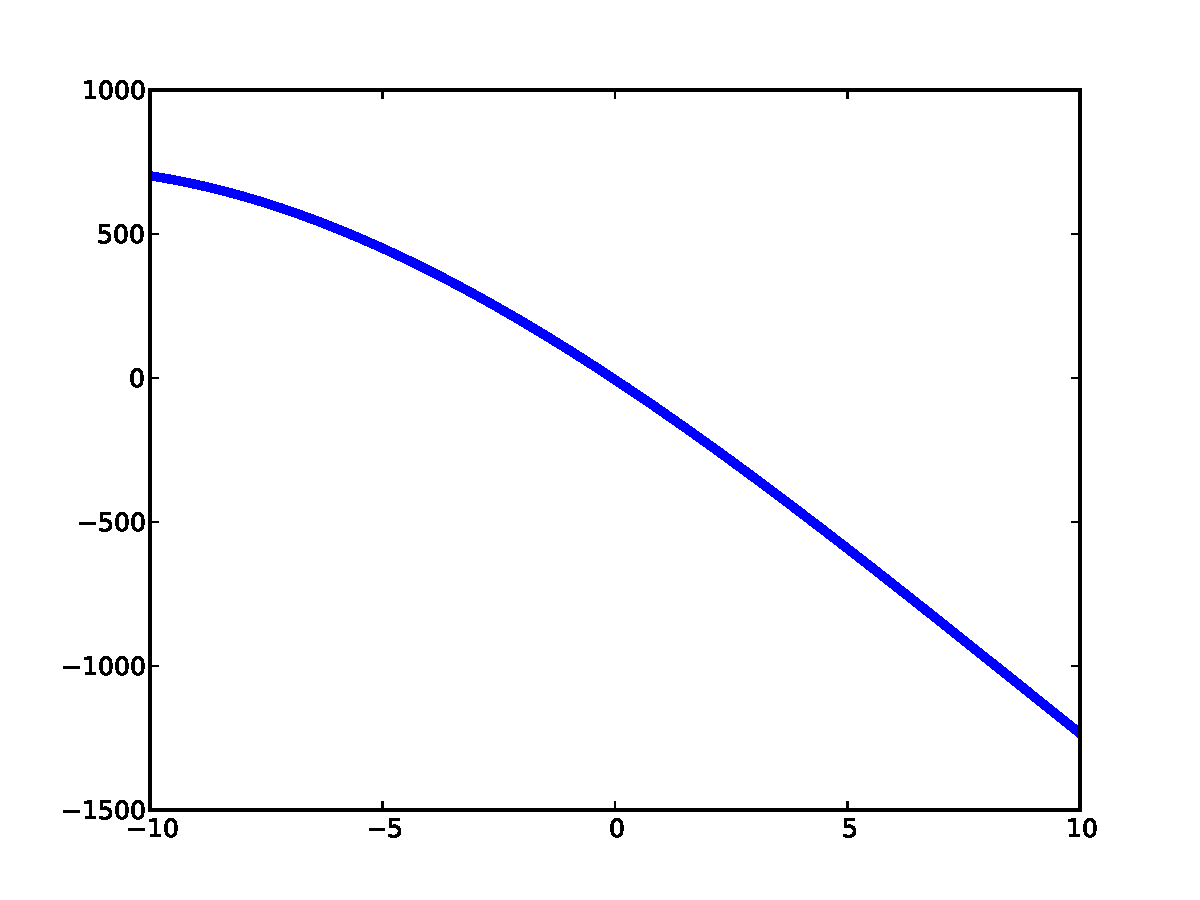
\includegraphics[width=.9\textwidth]{regression_f}
      }
      \only<2>{
        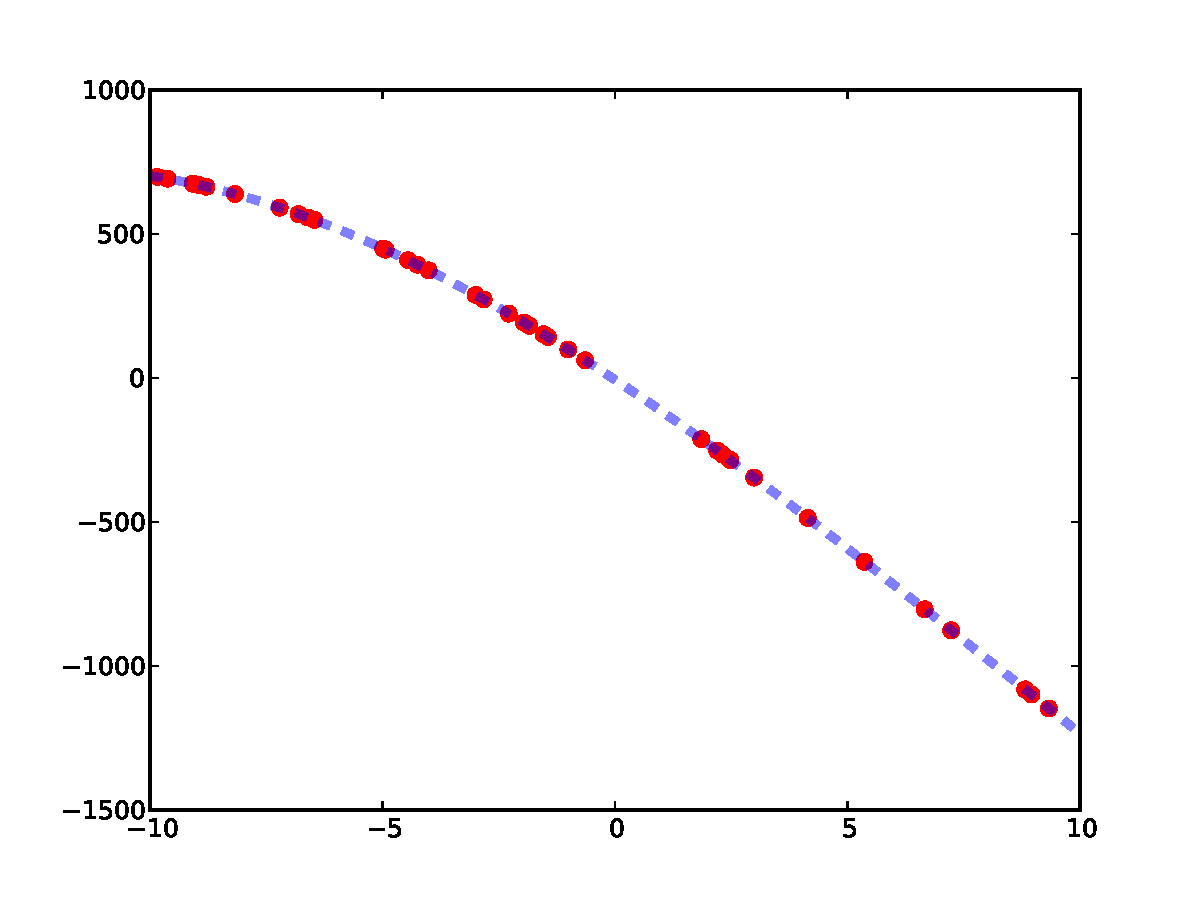
\includegraphics[width=.9\textwidth]{regression_obs}
      }
      \only<3->{
        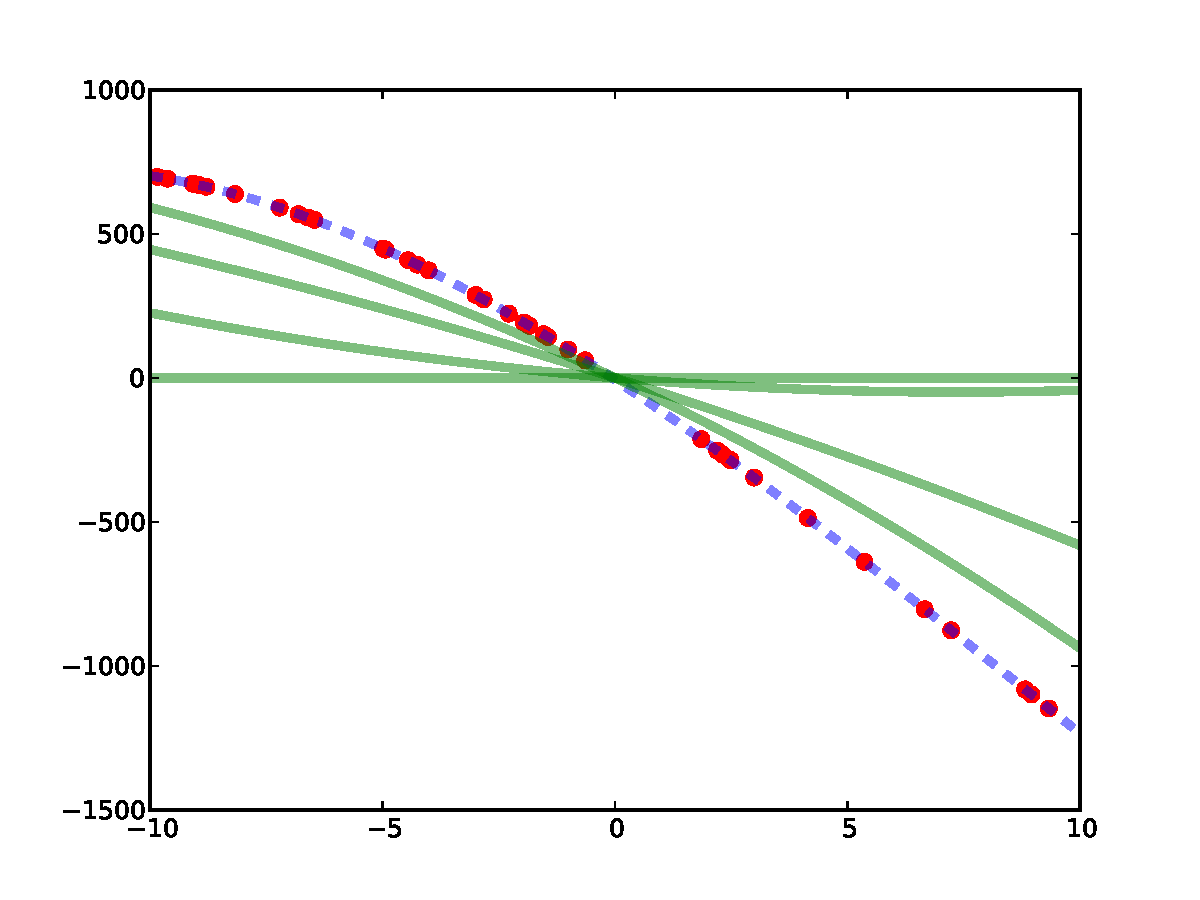
\includegraphics[width=.9\textwidth]{regression_several-thetas}
      }
  \end{figure}
    \end{column}
  \end{columns}
  \begin{itemize}
    \item<5-> Objectif : trouver $\theta^*$ solution de
      \[
        \min_{\theta \in \Theta} \hat{R}\left( \theta \right)
      \]
  \end{itemize}

\end{frame}

\begin{frame}
  \frametitle{Exemple}

  \begin{itemize}
    \item Exemple : estimation polynomiale
      \begin{itemize}
        \item $\hat{f} : (x; \theta) \mapsto \theta_0 + \theta_1 x + \theta_2 x^2$,
        \item $\hat{R}(\theta) = \frac{1}{2n} \sum_{i = 1}^n \left( \hat{f}(x_i) - f(x_i) \right)^2$
      \end{itemize}
    \item Qualit\'e d\'ependante du choix de $\hat{f}$
  \end{itemize}
  \begin{columns}
    \begin{column}{.5\textwidth}
      \begin{figure}
        \centering
        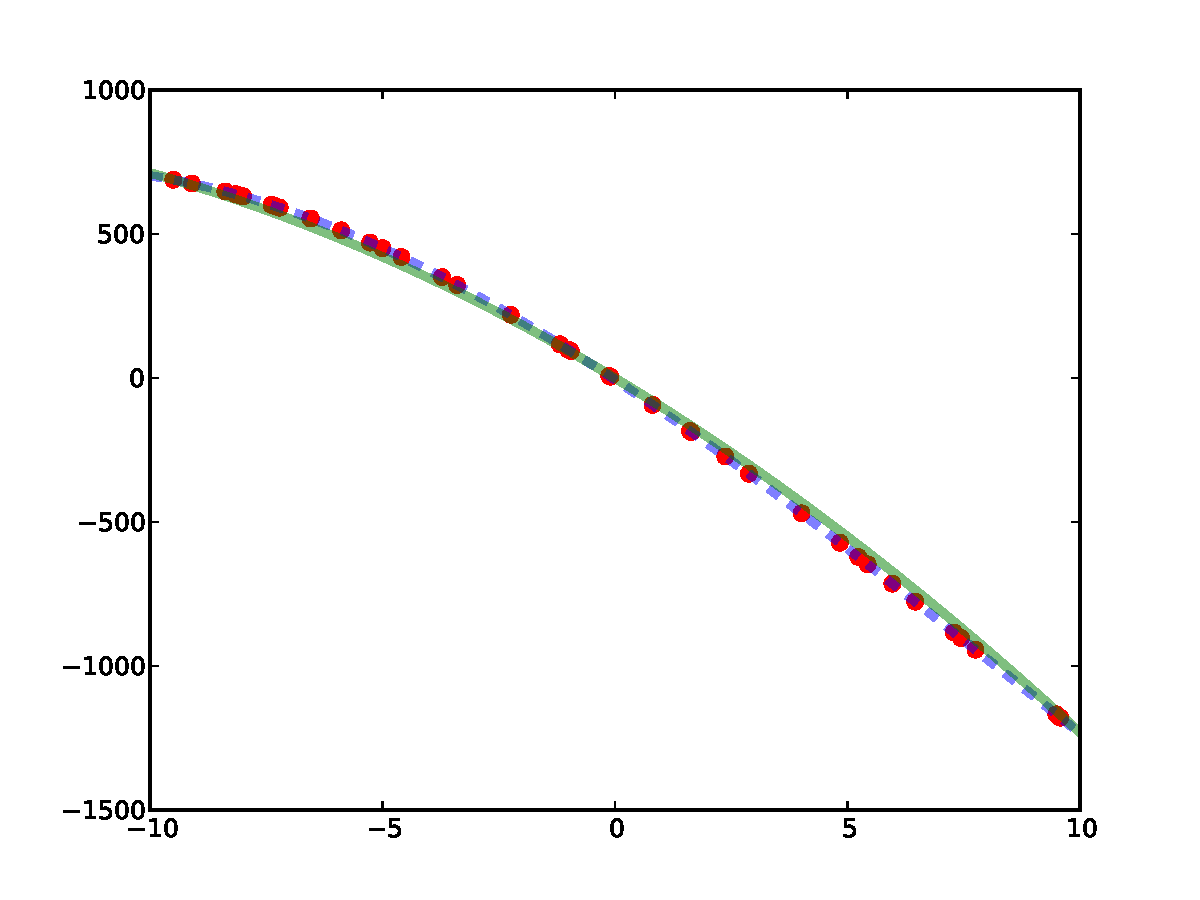
\includegraphics[width=.9\textwidth]{regression_good-choice}
        \caption{$\hat{f}$ adapt\'ee.}
      \end{figure}
    \end{column}
    \begin{column}{.5\textwidth}
      \begin{figure}
        \centering
        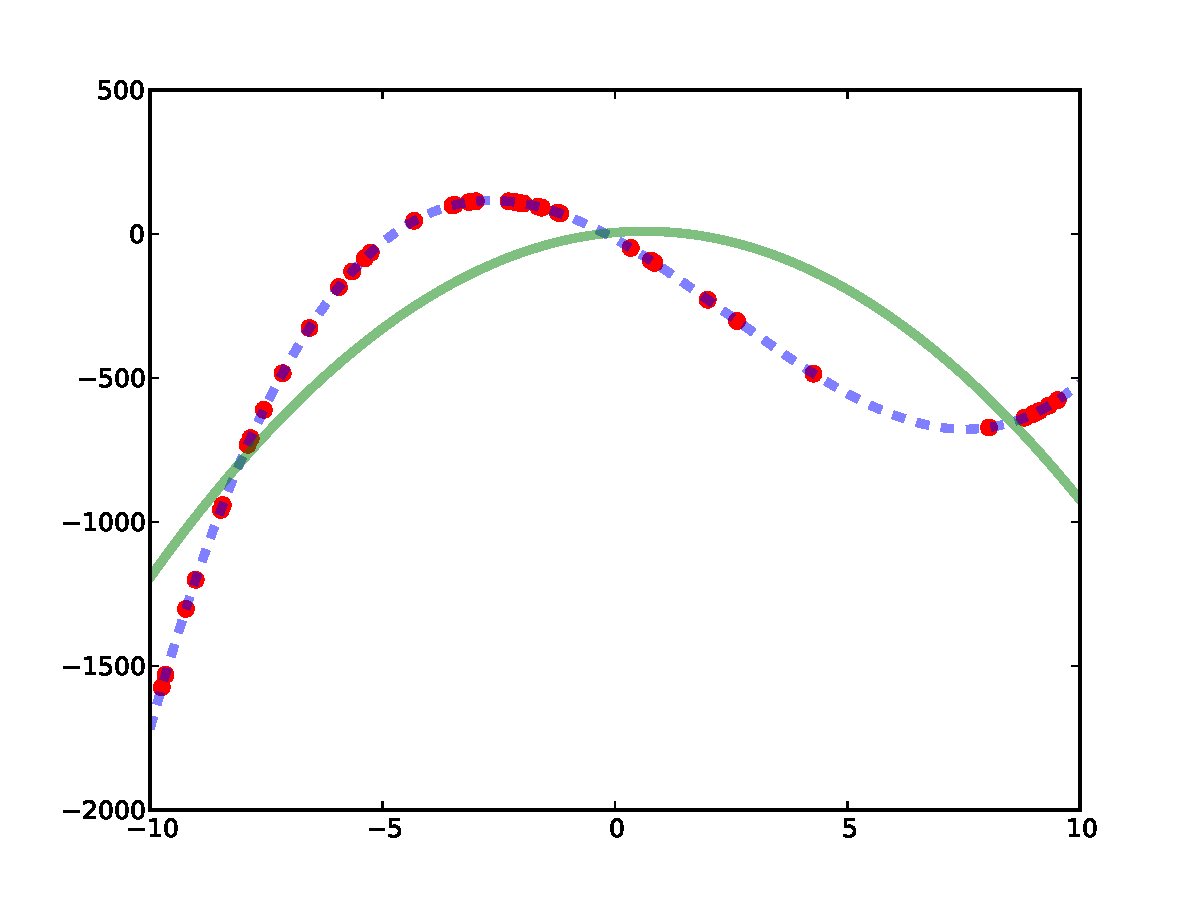
\includegraphics[width=.9\textwidth]{regression_poor-choice}
        \caption{$\hat{f}$ non adapt\'ee.}
      \end{figure}
    \end{column}
  \end{columns}
\end{frame}

\begin{frame}
  \frametitle{Application au problème initial}

  \begin{itemize}
    \item Fonction à estimer : $f : x \mapsto \mathbb{E}\left[ D(x,X) \Phi_P(x,X) \right]$
    \item Risque empirique : moindres carr\'es
    \item Estimateur à noyaux :
      \[
          \hat{f}(x; \mathbf{\theta}, \mathbf{w}, a) = a + \sum_{j=1}^m w_j K(x - \theta_j)
      \]
      où $K$ est un noyau gaussien.
  \end{itemize}
  \begin{columns}
      \begin{column}{.5\textwidth}
          \begin{figure}
              \centering
              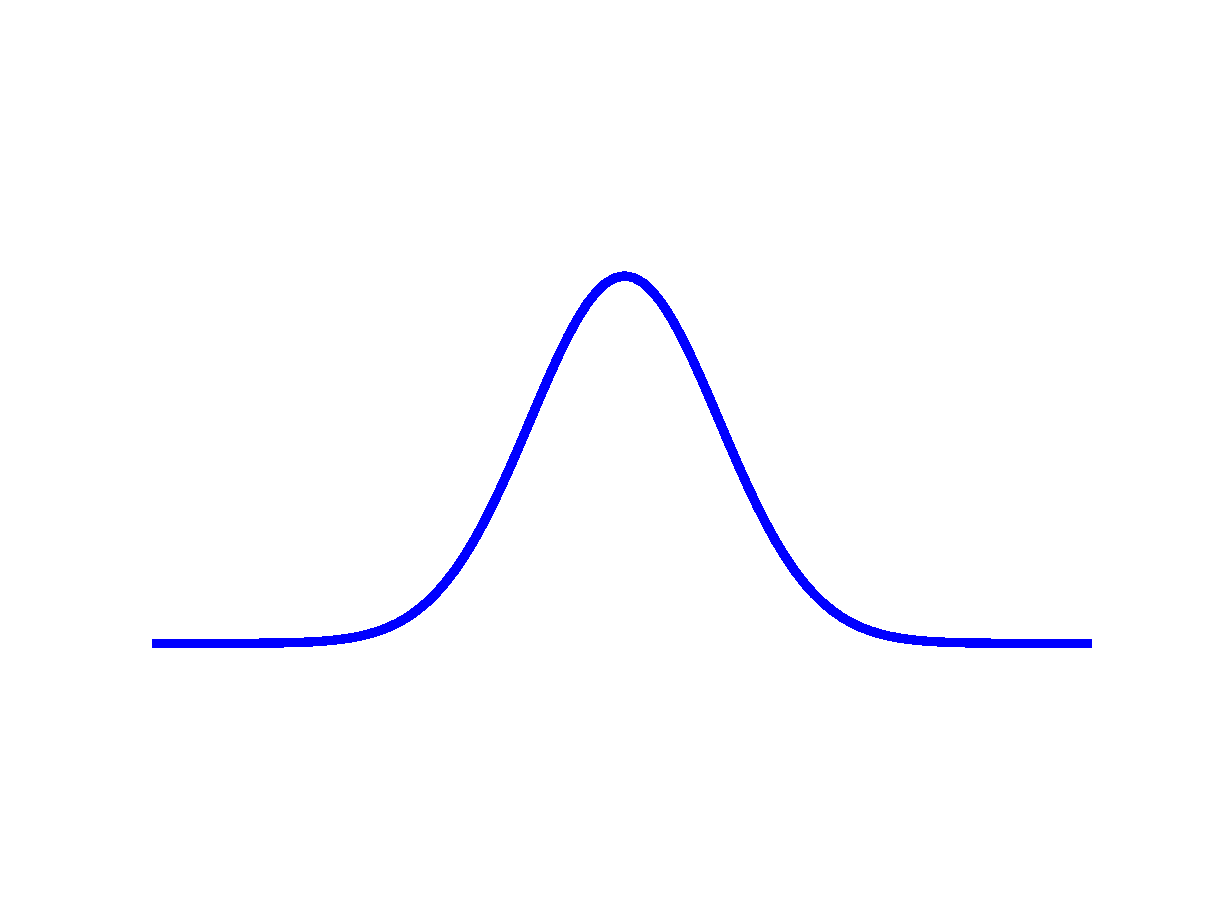
\includegraphics[width=.7\textwidth]{gaussian_kernel_1d}
              \caption{Noyau gaussien 1D}
          \end{figure}
      \end{column}
      \begin{column}{.5\textwidth}
          \begin{figure}
              \centering
              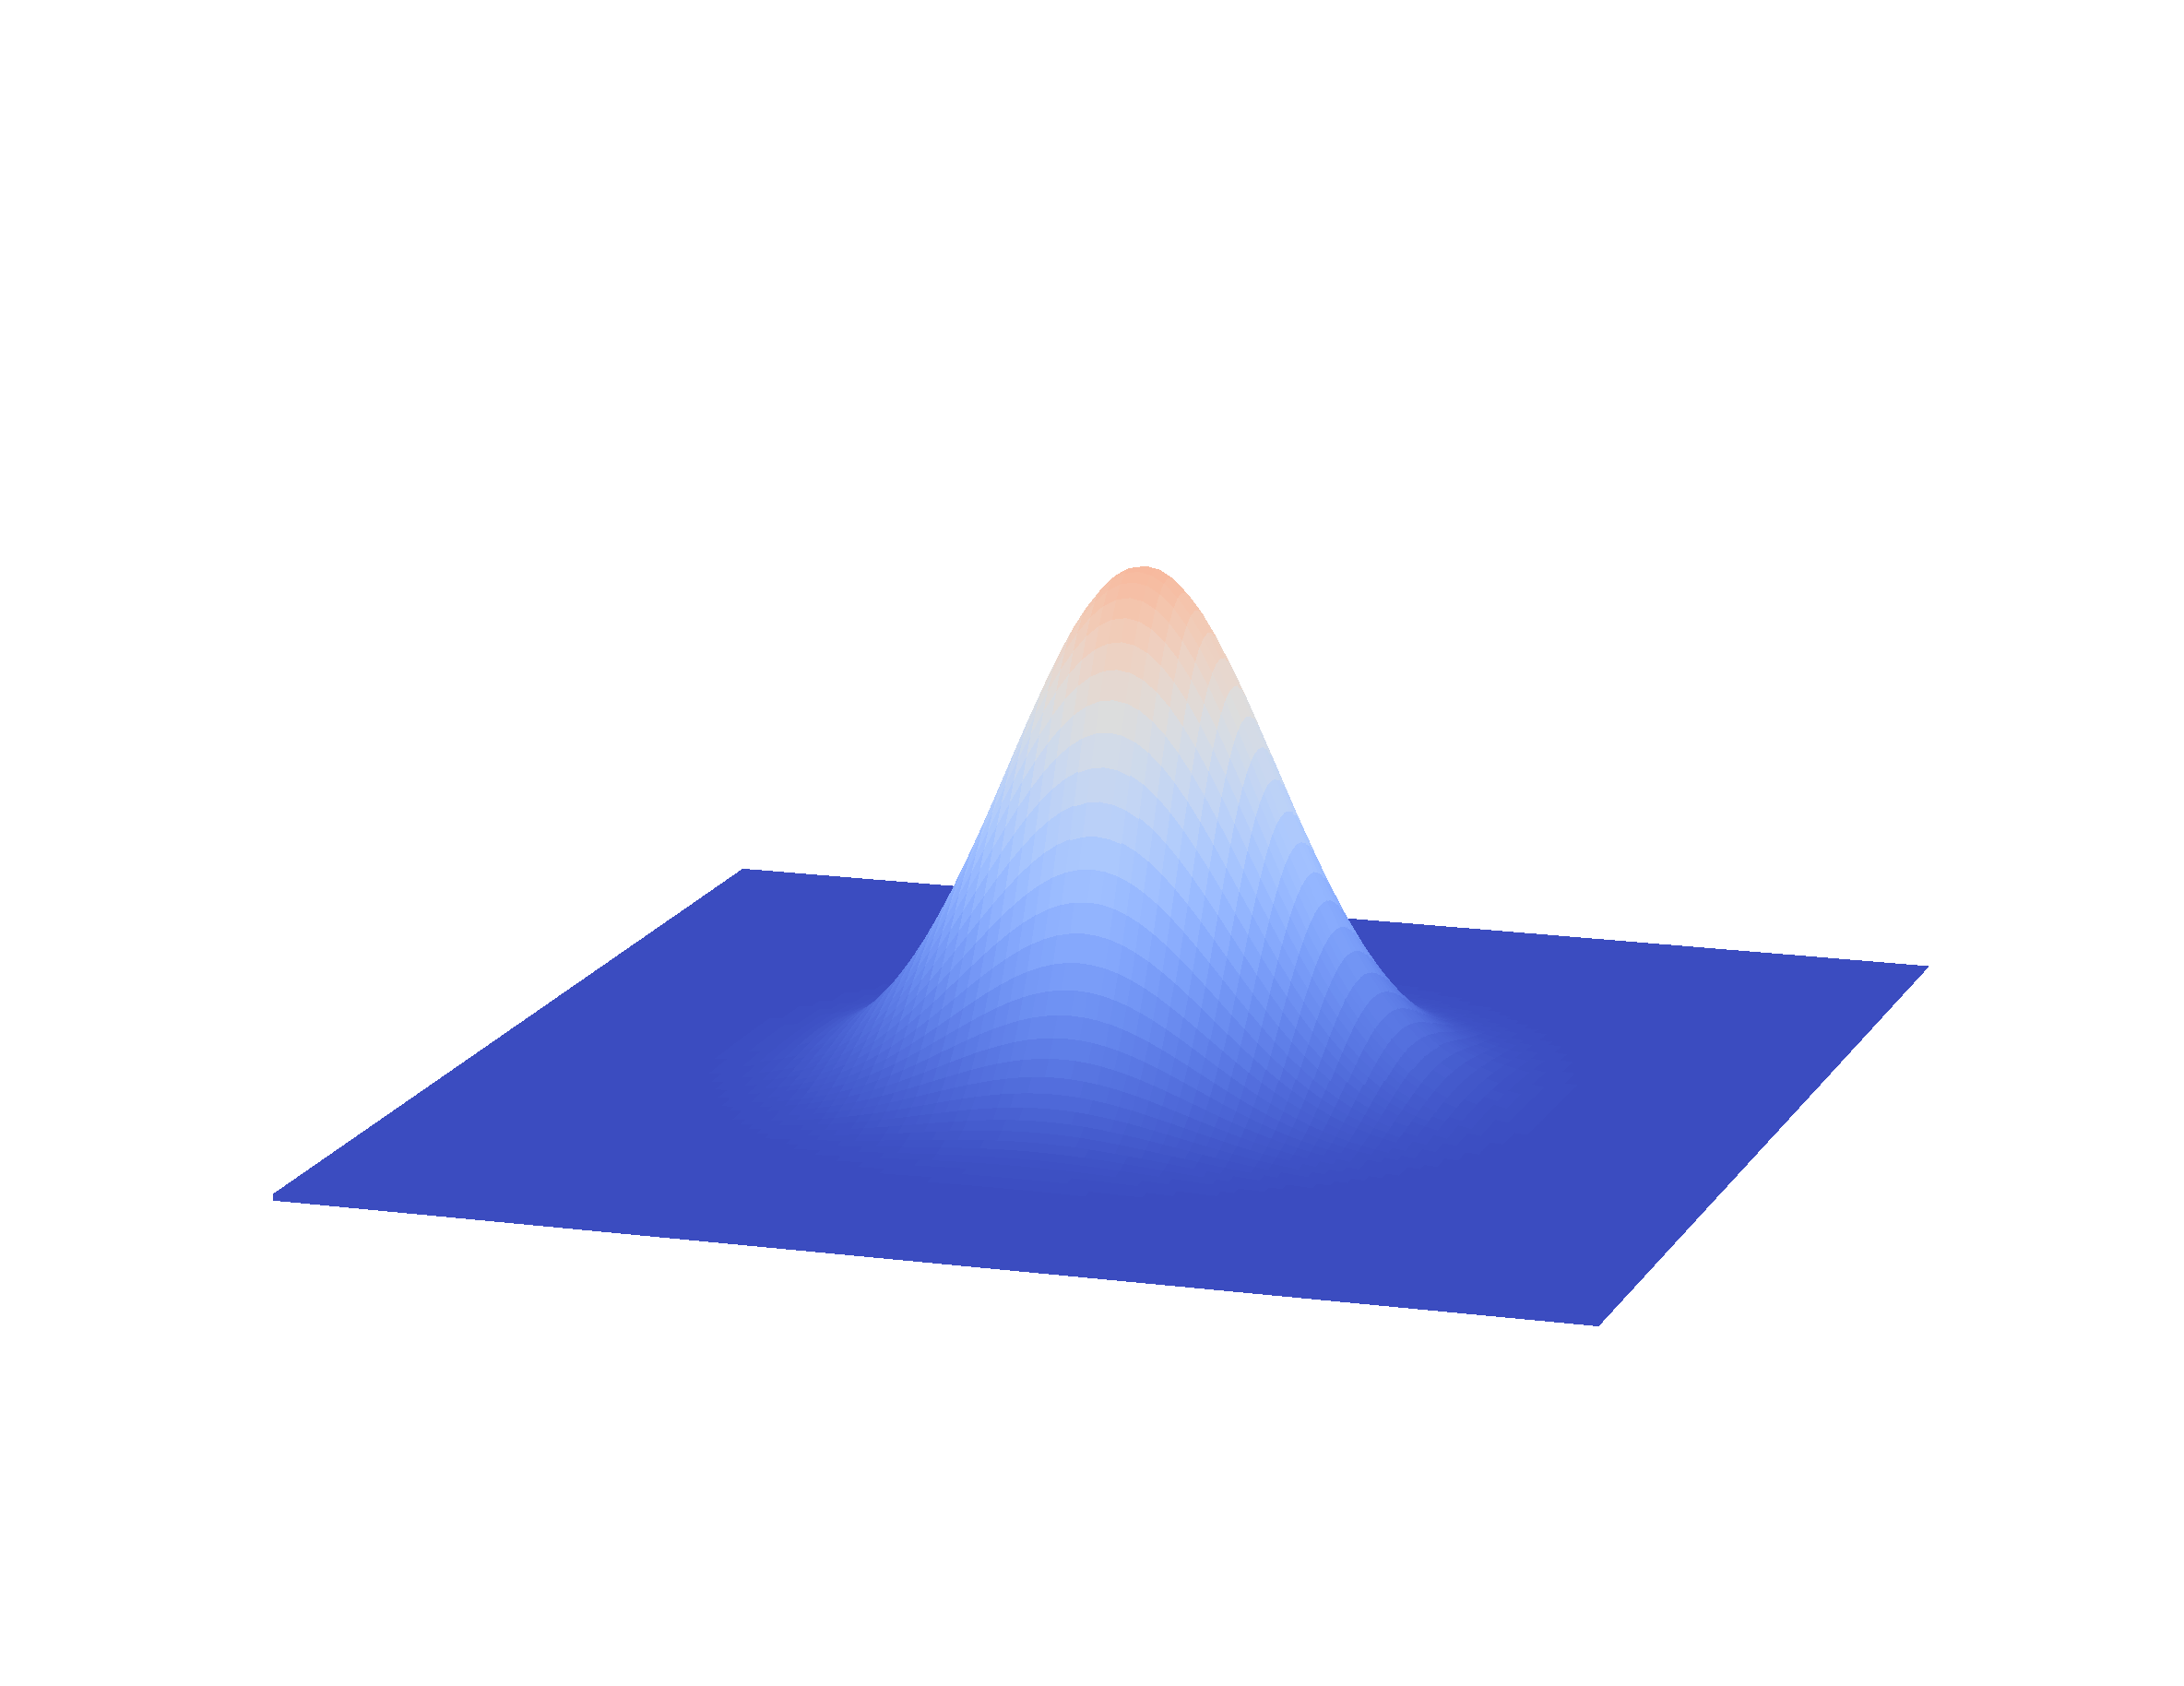
\includegraphics[width=.7\textwidth]{gaussian_kernel_2d}
              \caption{Noyau gaussien 2D}
          \end{figure}
      \end{column}
  \end{columns}

\end{frame}

\begin{frame}
    \frametitle{Résultats}

    \begin{itemize}
        \item Application :
            \begin{itemize}
                \item $D : (x, y) \mapsto \|x - y\|_2$
                \item $(X_i)_{1 \leq i \leq n}$ : $n$ tirages d'un mélange de gaussiennes
                \item Observations empiriques $\tilde{f}(x_i) = \frac{1}{n} \sum_{j=1}^n D(x_i, x_j) \Phi_p(x_i, x_j)$
            \end{itemize}
        \item Objectif :
            \[
                \min_{\theta, w, a} \hat{R}(\theta, w, a)
                = \frac{1}{2n} \sum_{i= 1}^n \left( \hat{f}(x; \theta, w, a) - \tilde{f}(x_i) \right)^2
            \]
    \end{itemize}
\end{frame}

\begin{frame}
    \frametitle{Résultats optimisation globale}

    \begin{figure}
        \centering
        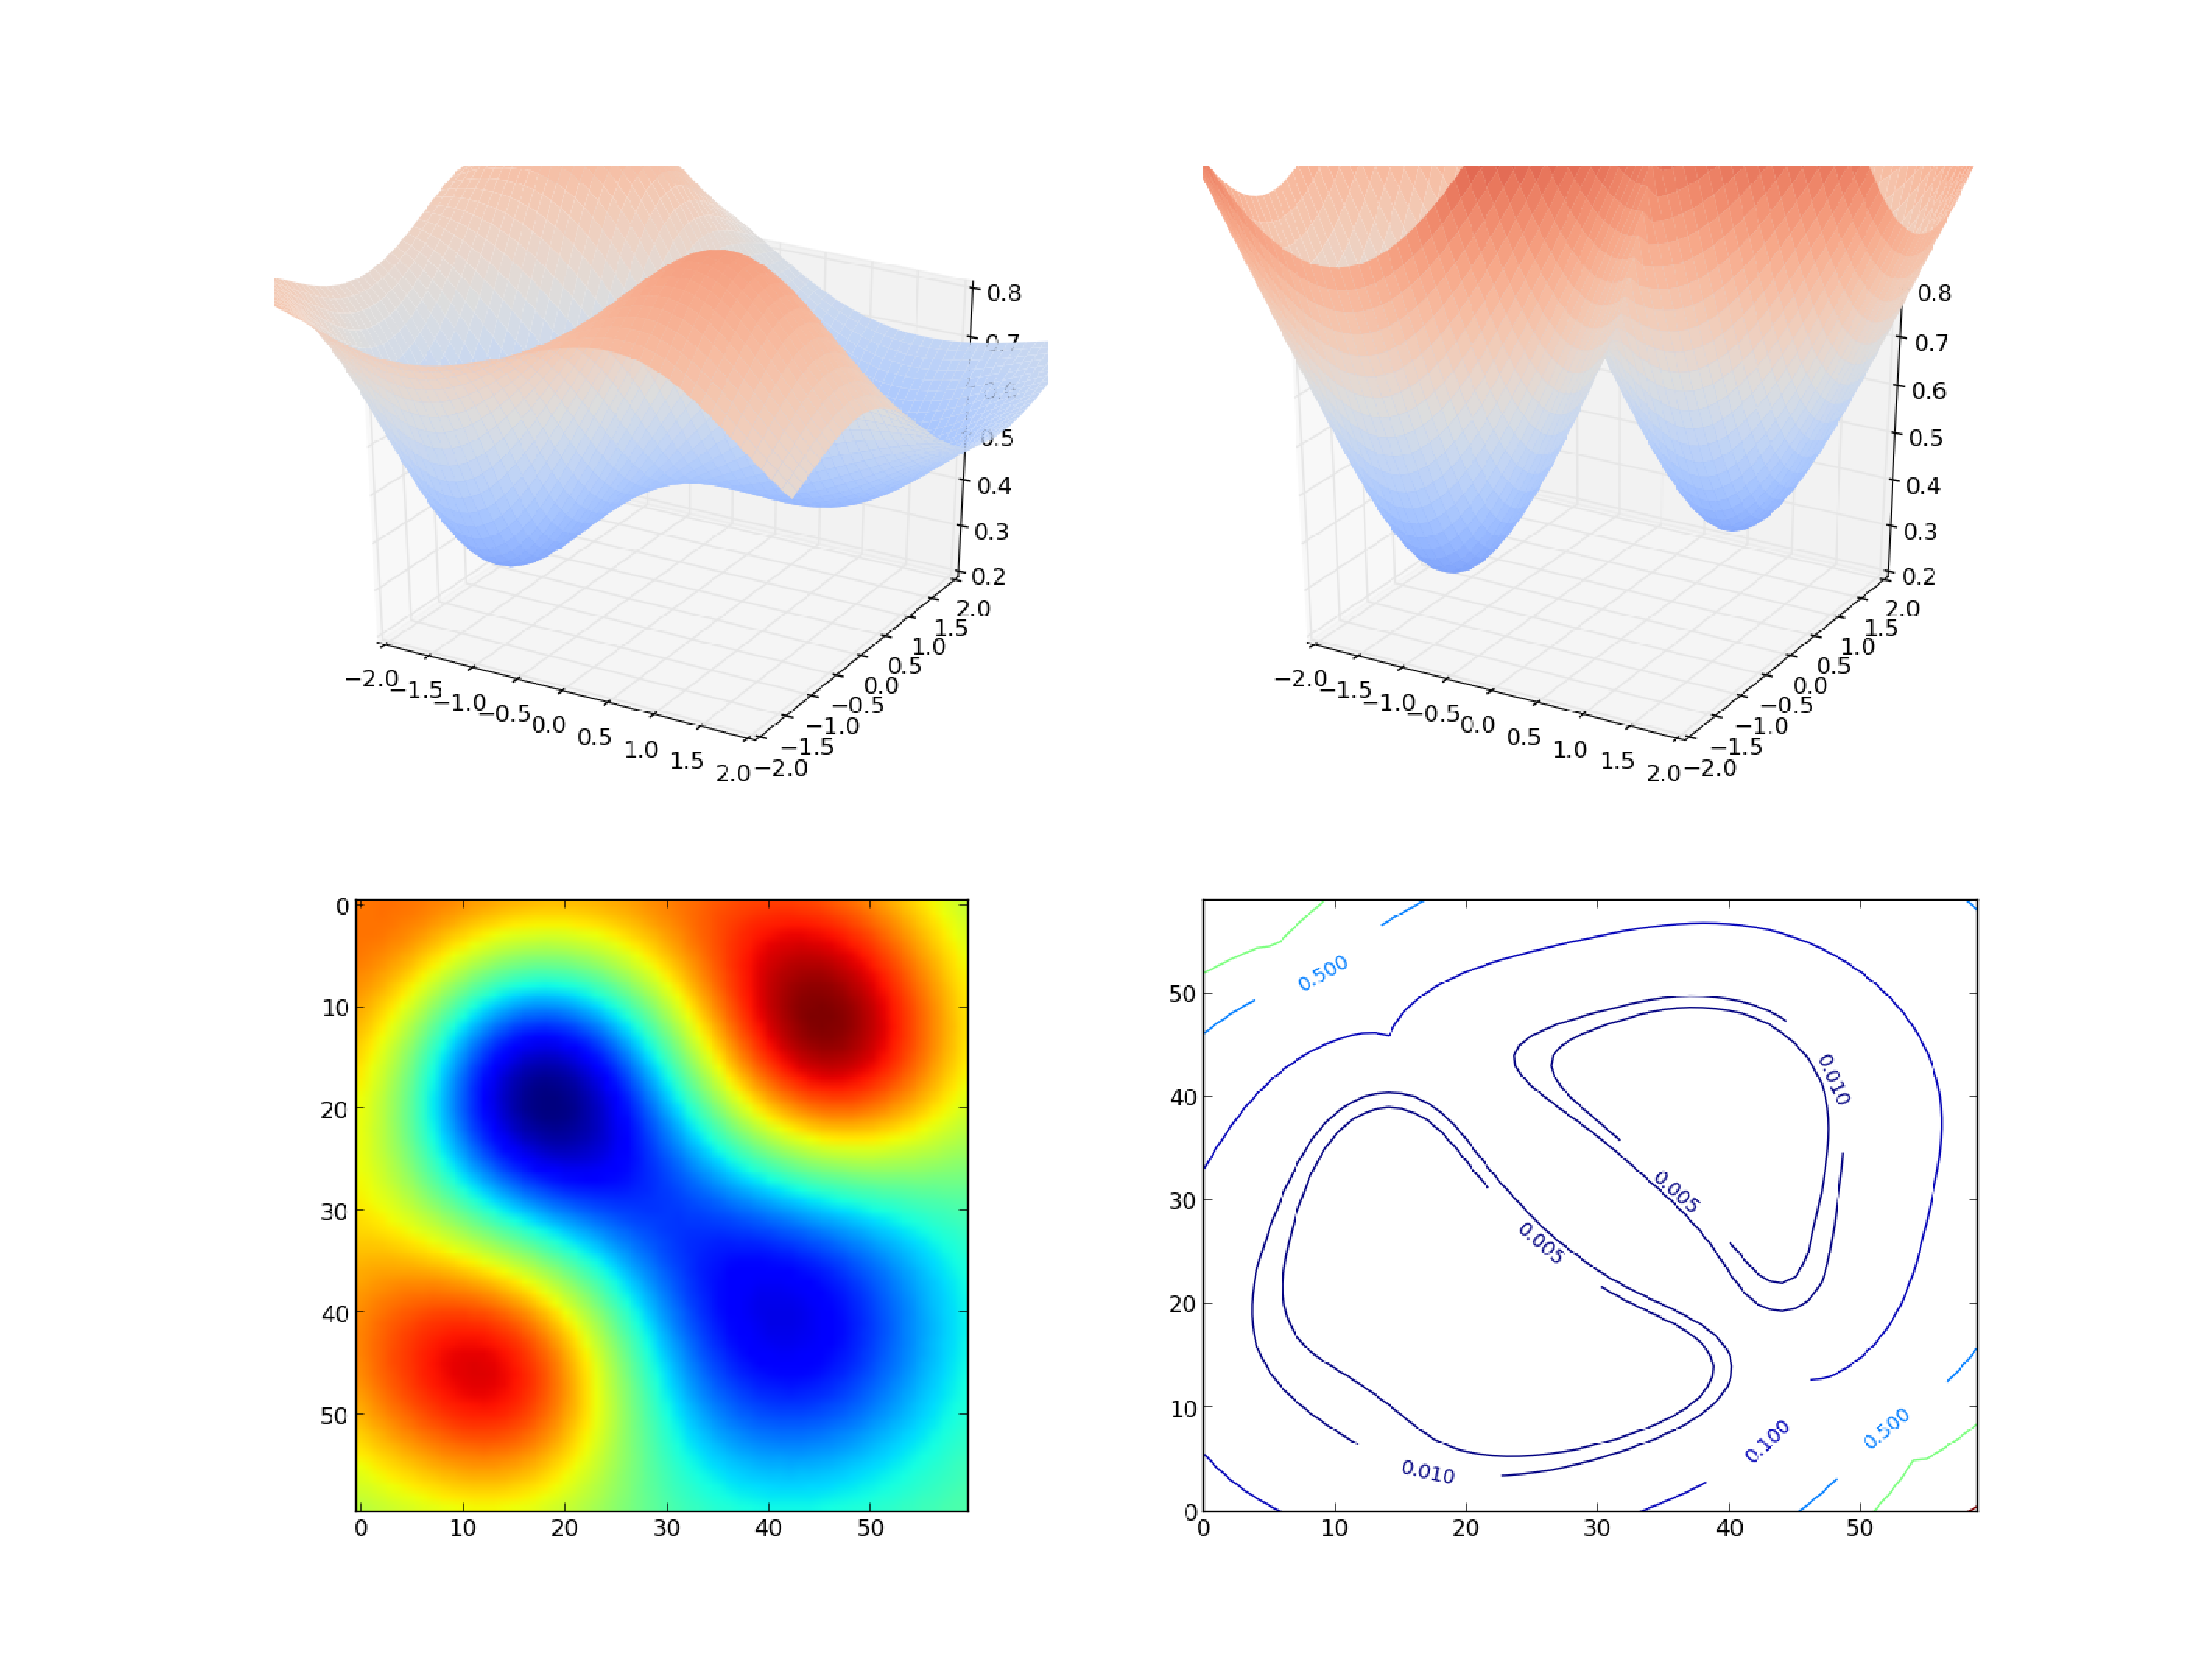
\includegraphics[width=.8\textwidth]{kernel_estimation_global}
    \end{figure}
\end{frame}

\begin{frame}
    \frametitle{Résultats optimisation distribuée}

    \begin{figure}
        \centering
        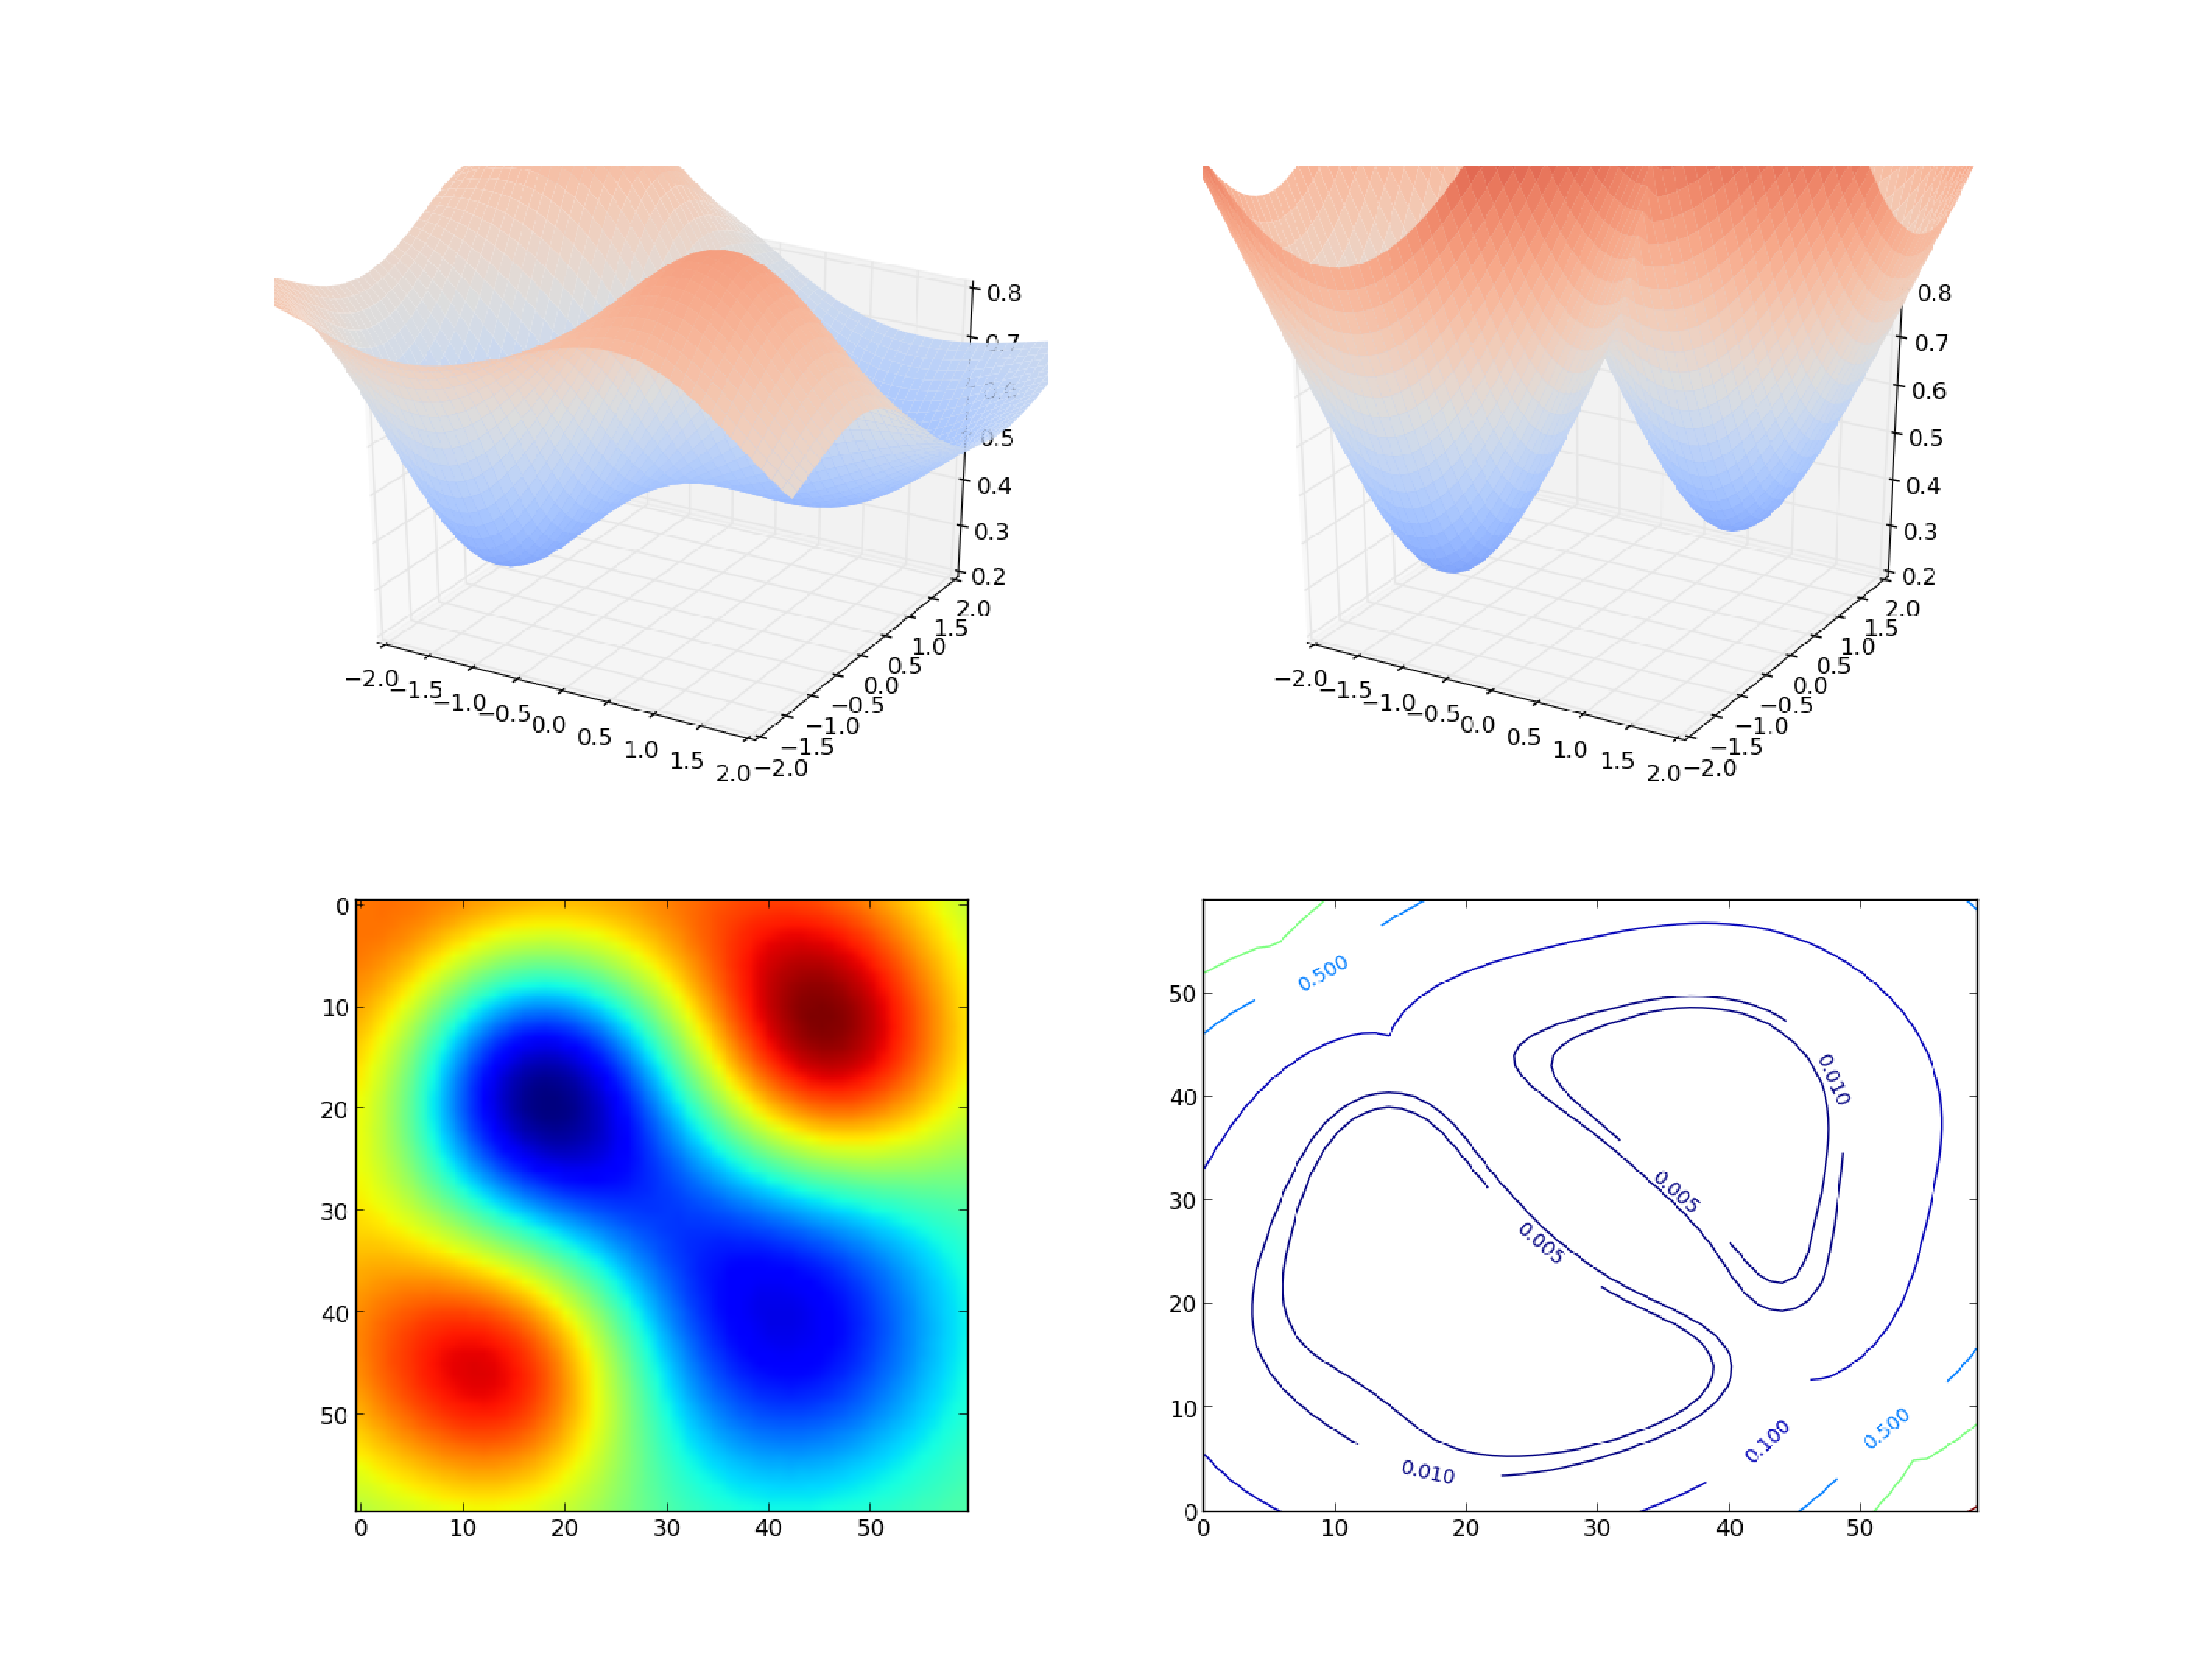
\includegraphics[width=.8\textwidth]{kernel_estimation_global}
    \end{figure}
\end{frame}

\begin{frame}
    \frametitle{Contrainte supplémentaire}

    \begin{itemize}
        \item $\tilde{f}(X_i)$ non accessible
        \item Idée : si l'agent $i$ a accès aux caractéristiques $(X_j)_{j \in \mathcal{A}_i}$
            ($i \in \mathcal{A}_i$), il peut :
            \begin{itemize}
                \item estimer la distribution des $X$ à partir des observations
                    accessibles
                \item utiliser le risque $R_i$ :
                    \[
                        R_i : (\theta, w, a) \mapsto \mathbb{E}_{\mu_i} \left[ \left( \hat{f}(x; \theta, w, a) - \mathbb{E}_{\mu_i}[D(x, X) \Phi_P(x, X)]\right)^2 \right]
                    \]
            \end{itemize}
        \item Le problème devient alors
            \[
                \min_{\theta, w, a} \frac{1}{n} \sum_{i = 1}^n R_i(\theta, w, a)
            \]
    \end{itemize}
\end{frame}

\begin{frame}
    \frametitle{Résultats}

\end{frame}

\end{document}
